% This file is part of the `speccal` project.
% Copyright 2014 the authors.
% All rights reserved.

% ## style notes:
% - all equations in `eqnarray` environments
% - use `\,` as the multiply operator!
% - parameters are `inferred`; `measurement` is reserved for data
% - use emulateapj or aastex, as you like, but watch for equation-wrapping in the former

% ---- Hogg (aastex) mode ----
%\documentclass[12pt, letterpaper, preprint]{aastex}
% ----


% ---- Charlie (emulateapj) mode ----
 \documentclass[iop,numberedappendix]{emulateapj}
 \usepackage{apjfonts}
% ----
\usepackage{color, hyperref}
\bibliographystyle{apj}
\input{vc}

% math shih
\newcommand{\transpose}[1]{{#1}^{\!\mathsf T}}
\newcommand{\given}{\,|\,}
\renewcommand{\det}[1]{||{#1}||}

% affiliation marks; edit with care
\newcommand{\lick}{1}
\newcommand{\ccpp}{2}
\newcommand{\cds}{3}
\newcommand{\mpia}{4}

%figures
\usepackage{graphicx}
\DeclareGraphicsExtensions{.png,.pdf}
\newcommand{\excluster}{B192-G242}

%references
\newcommand{\foreign}[1]{\emph{#1}}
\newcommand{\etal}{\foreign{et\,al.}}


\begin{document}\sloppy\sloppypar
\title{Combining information from photometric and spectroscopic data:\\
  Don't waste your time in spectrophotometric calibration!}
\shorttitle{don't waste your time in calibration!}
\author{
  BDJ\altaffilmark{\lick},
  DRW\altaffilmark{\lick},
  DFM\altaffilmark{\ccpp},
  DWH\altaffilmark{\ccpp, \cds, \mpia},
  CC\altaffilmark{\lick},
  others}
\shortauthors{bdj et al}
\altaffiltext{\lick}{University of California Lick Observatory}
\altaffiltext{\ccpp}{Center for Cosmology and Particle Physics, Department of Physics, New York University}
\altaffiltext{\cds}{Center for Data Science, New York University}
\altaffiltext{\mpia}{Max-Planck-Institut f\"ur Astronomie}

\begin{abstract}
In a typical spectral-fitting project,
  there tend to be a small number of bands of well-calibrated photometry
  and thousands of poorly calibrated spectroscopic pixels.
Good spectroscopic calibration is both expensive and difficult,
  but naive weighted least-square fitting will weight
  the thousands of spectroscopic pixels far higher overall
  than the few photometric bands.
Here we present a flexible and general spectroscopic calibration model,
  which can be fit simultaneously along with whatever spectral parameters.
The model involves a polynomial calibration vector to capture large-scale calibration issues
  and a Gaussian Process to capture small-scale wiggles.
We show that, in this framework, the quality of some kinds of spectral parameter fits
  is not a strong function of the quality of the spectroscopic calibration;
  that is, for many scientific goals there is no scientific reason
  to obtain good---or really any---spectrophotometric calibration.
In particular, for stellar population fitting, high signal-to-noise data,
  and good photometry,
  we show that raw counts are just as good as calibrated counts for making inferences about the
  parameters of interest.
This obviation of calibration overheads will pay \emph{all yall mad cheddar},
  at least if yall employ full cost accounting.
\end{abstract}

\keywords{
  greetings
  ---
  whole world
}

\section{Introduction}

In probabilistic inference, all information flows from the data to the
parameters of interest by means of a likelihood function, or an
expression for the probability of the data conditioned on the
parameters.
If there are $N$ independent sources of data, for each of which there
is a likelihood function, the full-data likelihood is the product of
the $N$ individual likelihoods (or the log-likelihood is a sum of the
$N$ individual log-likelihoods).
There is no bespoke ``weighting'' of the data that is justifiable in
this framework.
This creates some apparent paradoxes!
One is the following:

Imagine you have three photometric bands through which you have
observed some object (independently, say), and also a 2500-pixel
spectrum, where the pixels are defined such that they are precisely or
approximately independent measurements.
For these purposes, two spectral pixels are very close to independent
measurements if they are derived from disjoint sets of detector pixels
in the spectrograph detector plane.
Each photometric band and each spectroscopic pixel has a
log-likelihood function, and these 2503 log-likelihood functions must
be (by the Rules of Righteousness) coadded equally into one full-data
log-likelihood.
The log-likelihood is therefore fully dominated by the spectral
pixels!
This despite the fact that in almost all astronomical investigations,
the photometry is far more reliable, per measurement, than the
spectra.
That is, if the spectral pixels tend to prefer one model, or one set
of parameters, and the photometry another, the spectra will almost
always ``win'' just by their overwhelming numbers.

What is a Righteous Probabilistic Investigator (RPI) to do?
One option---fully unjustified---is to ``down-weight'' the
log-likelihoods of the spectral pixels relative to the photometric
measurements.
This is equivalent to taking the likelihoods to some power, which has
no justification in inference (though it is sometimes used in
optimization and sampling as an ``annealing'' move).
This down-weighting is not justified, but there is even more
ad-hockery than this, because there is no principled way to choose the
unprincipled weights.

The Right Thing To Do is to express the \emph{reason} that the RPI
believes the spectroscopic data to be less reliable \emph{within} the
likelihood function.
That is, the RPI must add nuisance parameters to parameterize the
unreliability of the spectroscopy, and infer those along with the
parameters of interest.
If this parameterization is good, the information in the spectroscopy
data will not flow entirely to the parameters of interest; instead,
some will flow to the nuisance parameters.
This will reduce the importance of the spectroscopy relative to the
photometry and the RPI will be well pleased with the dominance of the
photometric data in the final inferences of the parameters of
interest.
In what follows, we provide an example of this kind of
parameterization and inference.

Our example involves instantiating a ``calibration adjustment'' model,
which itself has both a polynomial component and a non-parametric
component.
The parameters of the calibration adjustment are nuisances, from a
scientific standpoint.
However, because the calibration adjustment is inferred along with the
parameters of interest, the probabilistic inference that provides
parameter estimates \emph{also} provides a spectrophotometric
calibration of the spectral data.
That is, the method we present has the potential to \emph{obviate
spectrophotometric calibration}.

We find that this potential---obviation of calibration---is realized.
That is, if the procedures demonstrated below become widely adopted,
some or perhaps most astronomical spectroscopic projects could
potentially drop or dramatically reduce their spectrophotometric
calibration programs.
This would reduce telescope overheads and data-analysis time and
complexity, delivering economic and sanity benefits to the whole
community.

\section{Model generalities}

THIS SECTION NEEDS WORK; THIS IS JUST AN EQUATION DUMP.

HOGG: A model is a parameterized likelihood function, with prior PDFs on the nuisance parameters (at least)...

HOGG: There is a likelihood for the photometry and for the spectroscopy...

HOGG: Each of these penalizes the difference between a column vector of data and a column vector of model expectation value...

The standard chi-squared or log-Gaussian log-likelihood is
\begin{eqnarray}
\ln p(d\given\theta) &=& -\frac{1}{2}\,\sum_{n=1}^N \left[\frac{[d_n - \mu_n(\theta)]^2}{\sigma_n^2} + \ln(2\pi\,\sigma_n^2) \right]
\quad ,
\end{eqnarray}
where $\theta$ is a blob of parameters of interest,
$d$ is the full set (in the form of a column vector) of data,
made up of $N$ values $d_n$,
$\mu(\theta)$ is the the column-vector mean prediction (expectation value) of the model,
made up of $N$ values $\mu_n(\theta)$,
the $\sigma_n^2$ are the observational noise variances.
We have included the $\ln(\sigma_n^2)$ term in the likelihood because
in what follows we are going to be modifying the noise model.

If you don't believe the reported data noise variances $\sigma_n^2$,
it often makes sense to add in quadrature a ``jitter'' variance $s^2$.
This is a trivial modification of the chi-squared log-likelihood:
\begin{eqnarray}\label{eq:photometricLF}
\ln p(d\given\theta,s^2) &=& -\frac{1}{2}\,\sum_{n=1}^N \left[\frac{[d_n - \mu_n(\theta)]^2}{[\sigma_n^2 + s^2]} + \ln(2\pi\,[\sigma_n^2 + s^2]) \right]
\quad .
\end{eqnarray}
This modification shows the necessity of including the log-variance
term.
This---equation~(\ref{eq:photometricLF})---is in fact the
log-likelihood function we are going to use for the photometric
measurements ({\color{blue} BDJ: IS THIS TRUE?} {\color{red} Jitter
will be added now with correct sign as I test increases in model
complexity }) in what follows.  
In this formulation, if $\theta$ are the parameters of interest, the
jitter variance $s^2$ is a nuisance noise-model parameter.  The
Gaussian Process will be a generalization of this modification.

We take the calibration-vector that modifies the mean model to produce
the observed spectrum as multiplicative with respect to the mean
model.  In this case we define the residual of the data from the model
in terms of the logarithmic differences.  This logarithmic formulation
requires that $d$ be everywhere positive, and distorts the
uncertainties, especially at low S/N ratio.  The advantages of
defining the residual in this way are that the model remains linear
(and therefore fast) and the calibration vector is forced to be
positive everywhere.  However, at high signal to noise the distortion
of the uncertainties will be minimal.

The calibration-vector and Gaussian-Process modified log-likelihood is
\begin{eqnarray}\label{eq:spectroscopicLF}
\ln p(d\given\theta,\alpha) &=& -\frac{1}{2}\,\left[\transpose{\Delta}\,C^{-1}\,\Delta + \ln([2\pi]^N\,\det{C}) \right]
\\
\Delta &\equiv& \ln d - \ln \mu(\theta) - f(\alpha) 
\\
C_{nn'} &\equiv& [\hat{\sigma}_n^2 + s^2]\,\delta_{nn'} +
K_\alpha(\lambda_n - \lambda_{n'})
\\
\hat{\sigma_n} & = &\sigma_n/d
\quad ,
\end{eqnarray}
where $\alpha$ is a blob of nuisance parameters
(which determine the jitter, the calibration vector and the kernel function),
$\Delta$ is a residual column vector,
$f(\alpha)$ is a calibration column vector,
$C$ is the Gaussian Process covariance matrix,
made up of $N^2$ values $C_{nn'}$,
$K_\alpha$ is a kernel function that sets the wavelength scale and
amplitude of the residual calibration issues,
$\hat{\sigma}_n$ are the fractional uncertainties of the data,
and each $\lambda_n$ is the wavelength of spectral pixel $n$.
The calibration vector $f(\alpha)$ is going to take care of the
large-scale calibration residual; the Gaussian process is going to
pick up smaller-scale residuals away from \emph{that}.
The residual column vector is defined in terms of the logarithmic
difference between the data and the mean model $\mu$ since we are
taking the calibration vector to be multiplicative with respect to
the mean model $\mu$. In this formulation the the mean model $\mu$ will be effectively
multiplied by $e ^{f(\alpha)}$ 
This---equation~(\ref{eq:spectroscopicLF})---is the log-likelihood we
are going to use for the spectroscopic data in what follows.

In detail, we are going to choose a $M$th-order polynomial form for
the calibration vector $f(\alpha)$ and a bell shape (Gaussian) for the
kernel function $K_\alpha(\cdot)$:
\begin{eqnarray}\displaystyle
f(\alpha) &=& c_0\,[1 + \sum_{m=1}^M c_m\,x^m]
\\
x &\equiv& \frac{\lambda}{\lambda_0} - 1
\\
K_\alpha(\lambda_n - \lambda_{n'}) &=& a^2\,\exp(-\frac{[\lambda_n - \lambda_{n'}]^2}{2\,\ell^2})
\\
\transpose{\alpha} &\equiv& \left[ \{c_m\}_{m=0}^M, s^2, a^2, \ell^2 \right]
\quad ,
\end{eqnarray}
where $\lambda$ is a column vector made up of the wavelengths $\lambda_m$
and $x$ is a scaled and shifted version of the same,
scaled by a fiducial wavelength $\lambda_0$.
Nuisance parameters $c_m$ set the shape of the large-scale calibration
issues, while $a^2$ and $\ell^2$ set the variance and correlation
length of the remaining covariant calibration noise.

\section{Experiments and Results}

We are now left to demonstrate that, by including photometry as well
as spectroscopy, it is possible to infer the parameters of interest
$\theta$ while marginalizing over the calibration parameters $\alpha$.
We will apply the methodology for spectrophotometric calibration
described above to \emph{actual, real} optical spectra of a stellar
clusters in M31.  Spectra of star clusters provide a good test case,
as they are less complex than galaxy spectra (for which it is
necessary to model the star formation history) but are by no means
trivial. In this way the key features of the calibration model and
methodology are not obscured.

To demonstrate the effectiveness of our strategy for combining
spectroscopic and photometric information we will infer the parameters
$\theta$ from a spectrum both \emph{before} and \emph{after} it has
been spectrophotometrically calibrated using typical techniques and
ancillary spectrophotometric calibration data.

\begin{figure}[h!]
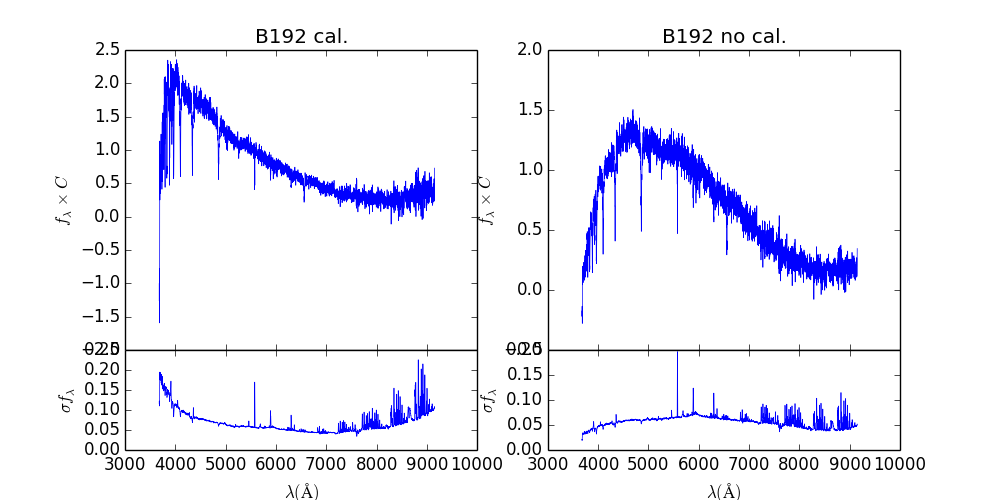
\includegraphics[width = 0.5 \textwidth]{figures/dfig_b192-g242_020.png}
\caption{The calibrated (left) and uncalibrated (right) spectrum for
\excluster, along with the uncertainties (bottom panel). The spectra
have been renormalized to avoid floating point errors. {\color{blue}
SHOULD THIS SHOW ALL THE CLUSTERS OR JUST ONE?.}\label{fig:data}}
\end{figure}

\subsection{List of Tests}

\begin{enumerate}

\item We should test on fake data, with known squiggly
  calibration applied, to demonstrate that we can infer the
  calibration vector and the physical parameters with no bias.  We
  should use the squiggly calibration derived from one of Nelson's
  calibrated/uncalibrated spectra.  We should also do this for
  differnt S/N to find where the logarithmic residual formulation
  breaks down.

\item We infer the parameters of the spectrum of a real cluster that
has been photometrically calibrated. Then, we infer the parameters of
the spectrum of the same cluster \emph{without} spectrophotometric
calibration, to see if we infer physical parameters consistent with
the calibrated case.  How many/which figures to show?

\item  Then, we show select marginalized or joint PDFs for many
clusters calibrated/uncalibrated, to assess consistency.  Or we just
show comparisons of confidence intervals for the parameters of a
number of clusters, calibrated/uncalibrated.

\item We infer the parameters of the calibrated spectrum without
including the noise model, or presumably the photometry (since
reconciling photometry and spectroscopy is done by our noise model).
What changed, what did we get wrong without the noise model?
{\color{blue} Should we keep the $f(\alpha)$ and the photometry?  This
just has the potential to show shortcomings in the spectrophotometric
calibration}

\item Finally, we change the number of photometric bands and see what
happens to the inferred parameters, using the full model.

\end{enumerate}

\subsection{Test Data}

The data we use to test our method consist of optical spectroscopy of
XX stellar clusters in M31 for which YY-band HST photometric data
exist.  The optical spectra were obtained using the fiber-fed
Hectoscpec intrument on MMT by \citet{caldwell}.  The wavelength range
of the spectra is $3700-9100$\AA. The instrumental resolution is
$\sim 5$\AA~ across the optical range \citep{fabricant13}.  {\color{blue} Wavelength
calibration happened. Sky subtraction happened.} The data were
approximately spectrophotometrically calibrated using an average
calibration vector for the night constructed from {\color{blue} MORE
HERE. Discuss S/N, sky subtraction.}


An example spectrum, both after and before spectrophotometric
calibration, is shown in Figure \ref{fig:data}.  When fitting the
spectra we mask the region around the bright OI5577 sky line, and we
fit only to the spectrum with $3750 < \lambda < 7200$\AA~ to avoid the low
S/N edges and, on the red side, imperfect sky line subtraction in a
region of the spectrum that has a paucity of informative spectral
lines. Furthermore, the MILES spectral library (see
\S\ref{sec:cluster_model}) only extends to $\lambda < 7500$\AA.
{\color{red} Specify/Justify order of calibration polynomial here?}.

{\color{blue} DRW words about photometry}

\begin{table}[h!]
\caption{List all the clusters, RA, Dec, photometry and individual exposures.}
\end{table}

\subsection{Star Cluster Model}
We model the stellar cluster as a single age SSP. The spectrum of a
star cluster under this assumption is given by
\begin{eqnarray}\displaystyle
F_{\theta^\prime}(\lambda_o) & = &
\frac{m_*}{4\pi d_L^2(1+z)} \, S(\lambda, t, Z , \beta) \, e^ {-k_\lambda\tau_V} \\
\nonumber \\ 
\lambda_o & = & (1+z)\,\lambda 
\\
\theta^\prime & \equiv & \left[ m_*, t, Z, \tau_V, z, d_L, \beta \right]
\quad ,
\end{eqnarray} where the
parameters $\theta^\prime$ include 
the stellar mass $m_*$, 
effective optical depth to dust in the $V$-band $\tau_V$, 
luminosity distance $d_L$,
and redshift $z$.  
The observed frame wavelengths $\lambda_o$ are related to the restframe
wavelengths $\lambda$ in the usual way.

The spectrum of one solar mass of stars that formed at lookback time
$t$ with metallicity $Z$ is given by $S(\lambda, t, Z [, \beta])$.
Here the additional parameters $\beta$ may include details of the
population synthesis model, such as the IMF slope and adjustments to
the stellar spectra or stellar evolutionary tracks. We will assume
$\beta$ to be fixed for the purposes of this exercise, with no loss of
generality {\color{blue} (KEEPING IMF SLOPE CONSTANT)}.  We will also
fix the shape of the attenuation curve, $k_\lambda \equiv
\tau_\lambda/\tau_V$, to the Milky way average of \citet{CCM89} with
$R_V=3.1$ and assume that $d_L$ is known to high precision from
independent methods and can therefore be treated as fixed.  In
practice, $d_L$ is completely degenerate with $m_*$. We calculate
$S(\lambda, t, Z)$ using the Flexible Stellar Population Synthesis
code \citep[FSPS][]{fsps}.  We use the Padova 2007 isochrones
\citep{girardi00, bertilli94, marigo07} and the MILES stellar spectral
library \citep{miles_I, miles_II, miles_III}.

The model spectra $F_{\theta^\prime}$ are smoothed by convolution
with a Gaussian in wavelength space (in this case to model the MMT
line-spread function) and are interpolated to the wavelength points of
the of the observed spectrum while taking into account the
redshift. The instrumental resolution is given by the parameter
$\sigma$.  {\color{blue}Discuss intrinsic resolution of model spectra
(MILES), what to do in situations where instrumental resolution is
higher, lower or comparable (ouch) to intrinsic velocity broadening.}

Nebular emission lines (which may arise from HII regions around the
clusters or from diffuse ionized gas) and interstellar absorption
lines are modeled as a sum of Gaussians of unknown amplitude $A_\ell$,
all of the same width $\sigma_e$ (which need not be the same as
stellar broadening $\sigma$) and with known central wavelengths
$\lambda_\ell$.  For emission lines the amplitudes are constrained to
be positive, while for interstellar absorption (e.g. Na D and Ca K)
the amplitudes are constrained to be negative. This framework can be
easily extended to include more complex models for the nebular
emission, such as allowing line dependent widths and velocities, and
using Voight profiles for the line shapes.  

The final mean model is then given by 
\begin{eqnarray}\label{eq:MeanModel} 
\mu(\theta) &  = & (G_\sigma  \otimes F_{\theta^\prime})(\lambda) +
\sum_{\ell=0}^{N_\ell} S_\ell(\lambda) \\
S_\ell (\lambda) & = & \frac{A_\ell}{\sigma_e\sqrt{2\pi}} \exp(-\frac{(\lambda -
 \lambda_\ell)^2}{2\sigma_e^2})\\
\theta & \equiv & \left[ \{\theta^\prime\}, \sigma, \{A_\ell\}_{\ell=0}^{N_l},
  \sigma_e \right]
\quad ,
\end{eqnarray}
where $G_\sigma$ represents a Gaussian of unit area 
and standard deviation $\sigma$, 
$\otimes$ indicates convolution, 
and the full parameter set $\theta$ now includes
the instrumental wavelength broadening $\sigma$ 
and the dispersion $\sigma_e$ and
amplitudes $A_\ell$ of the $N_l$ nebular emission and interstellar
absorption lines.
This is the mean model which appears in equation
\ref{eq:spectroscopicLF}.

To model the photometry we simply project the observed frame mean
model spectrum (equation \ref{eq:MeanModel}) onto the filters of
interest.  Note that we do \emph{not} include the calibration vector
$f(\alpha)$ in this projection.


\subsection{Sampling and Priors}

We estimate the posterior through MCMC sampling after an initial round
of optimization using Powell's method.  The specific sampling
algorithm we use is the affine-invariant ensemble sampling scheme of
\citet{goodman}, as implemented in the \texttt{emcee} package \citep{emcee}
Unlike typical Metropolis-Hastings MCMC sampling, the affine-invariant
sampler does not require the specification of step sizes in each
dimension.  {\color{blue}ASSESSING SAMPLER CONVERGENCE}
 
Our prior distributions are in all cases top-hat functions, described
in Table \ref{tbl:priors}, though more informative prior distributions
may be used.  Informative priors may be especially appropriate for the
calibration parameters $\alpha$ if additional information about the
instrument is available; or for the parameters of interest $\theta$,
for example in the case that there is knowledge of the metallicity
distribution of the population from which a given cluster is drawn.

\input{tables/priors.tbl}

\begin{figure*}[h!]
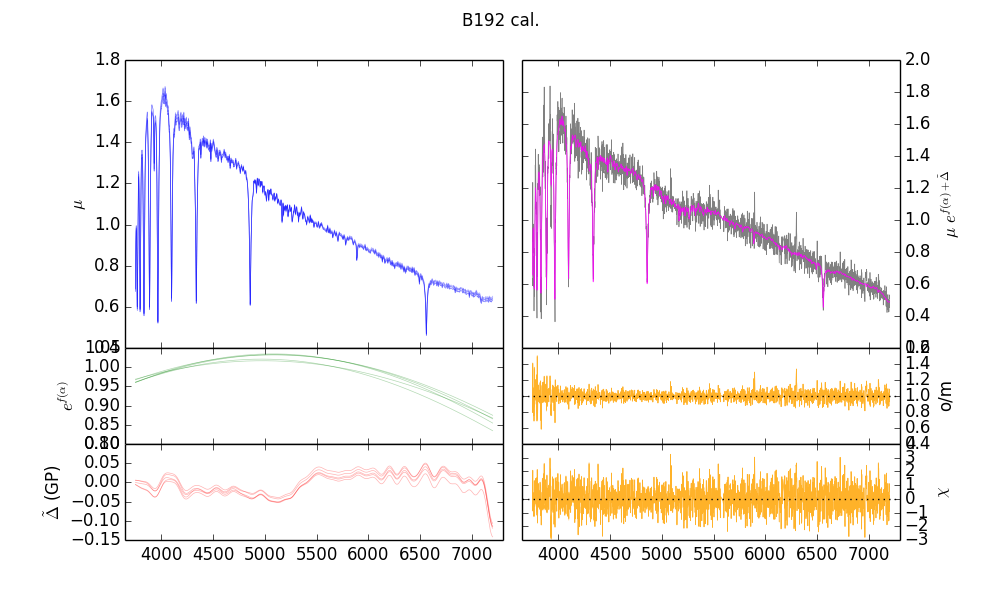
\includegraphics[width=\textwidth]{figures/sfig_b192-g242_225_cal.png}
\caption{Spectra resulting from draws from the posterior parameter
space conditioned on the calibrated \excluster~ spectrum and
photometry.  Left: For each of 5 draws from the posterior we show from
top to bottom, three components of the model: the mean cluster
spectrum, the calibration vector, and the mean prediction of $\Delta$
for the Gaussian process.  Right: From top to bottom, the full model
({\it magenta}) compared to the observed, calibrated spectrum ({\it
grey}), the ratio of the observed to the modeled spectrum, and the
difference between the observed spectrum and the modeled spectrum
normalized by the uncertainty.
\label{fig:inferred_spectrum}}
\end{figure*}

\begin{figure*}[h!]
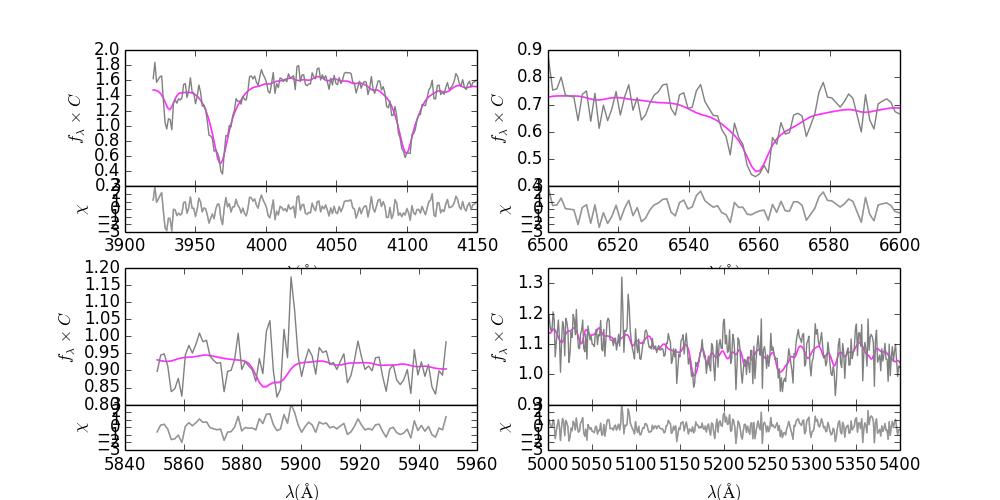
\includegraphics[width=\textwidth]{figures/zfig_b192-g242_225_cal.png}
\caption{Zoom-in on selected regions of the observed spectrum, showing
also draws from the posterior model for the spectra in these regions
and residulas of these draws from the observations.
\label{fig:zoom_spectrum}}
\end{figure*}

\subsection{Results}

We first infer the parameters of interest $\theta$ for a calibrated
spectrum of one of the clusters, \excluster, using the full YY-band
photometry. In Figure \ref{fig:inferred_spectrum} we show the spectra
that result from draws of the parameters $[\theta,\alpha]$ from the
posterior distribution, as well as several of the individual
components of the model constructed from each draw. Figure
\ref{fig:inferred_spectrum} also shows the calibrated spectrum on
which the priors were conditioned, and residuals between the posterior
models and the observed data.  The agreement is quite good, though
some lines are not accurately predicted.  For example, the observed
Mg$b$ absorption appears stronger than the modeled
absorption.

In Figure \ref{fig:inferred_sed} we show the corresponding SED for the
posterior parameter draws, compared to the observed SED. There is some
tension between the modeled and observed SEDs, I'm not quite sure
why. Finally, In Figure \ref{fig:inferred_params} we show the
marginalized and joint PDFs for a subset of the full model parameters.


\begin{figure}[h!]
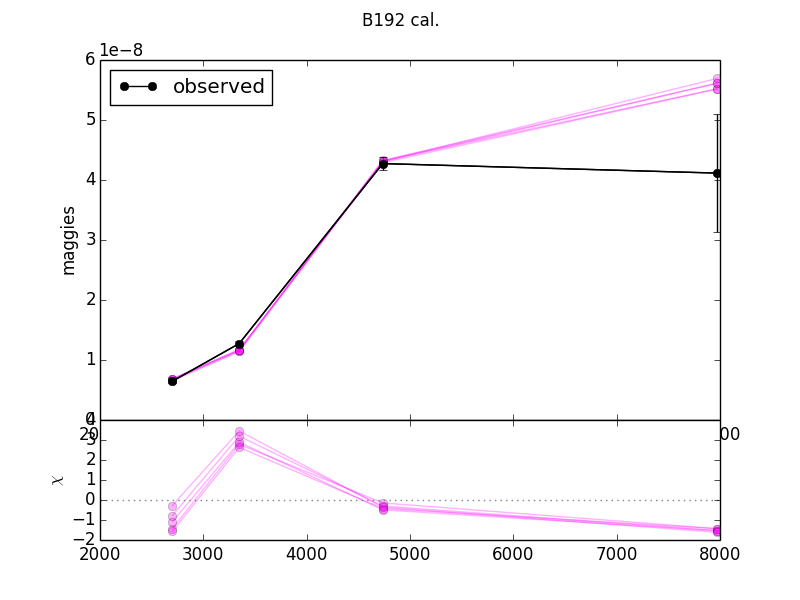
\includegraphics[width=0.5\textwidth]{figures/pfig_b192-g242_225_cal.png}
\caption{ Model SEDs.  Top: The model photometric SED resulting from
draws from the posterior parameter space conditioned ({\it cyan}) on
the observed photometry ({\it magenta}) and spectra.  Bottom:
uncertainty normalized residuals of the models from the observations.
\label{fig:inferred_sed}}
\end{figure}

\begin{figure}[h!]
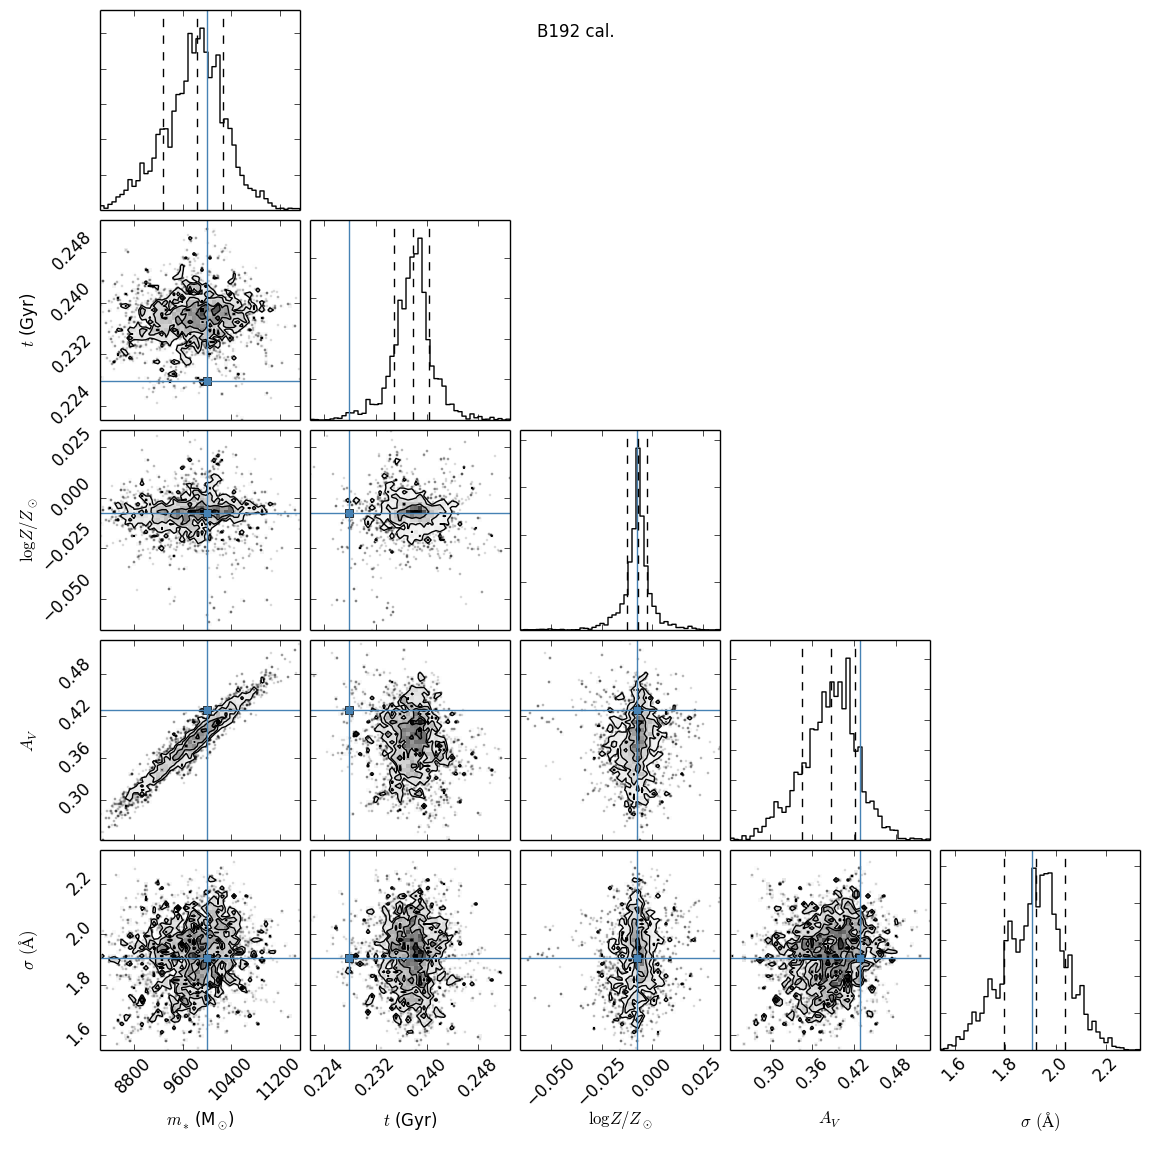
\includegraphics[width=0.5\textwidth]{figures/ptri_b192-g242_225_cal.png}
\caption{ Marginalized and joint PDFs of subset of the physical
parameters $\theta$ inferred from the spectophotometrically calibrated
spectrum of \excluster. The blue lines indicate the parameter values
that resulted from the powell minimization.
\label{fig:inferred_params}}
\end{figure}

The physical model parameters that we infer indicate that \excluster~
has super-solar metallicity, an age of $\sim 225$ Myr, moderate dust
extinction, and a stellar mass of $\sim 10^{4}$ M$_{sun}$ {\color{blue}
check that this is current mass, not initial mass}.  We find a spectral
broadening of $\sim 1.75$\AA~ (4.1\AA~ FWHM), which when combined in
quadrature with the intrinsic resolution of the MILES library, 2.5\AA~
FWHM \citep{beifiori11}, reproduces the typical line-spread function
of the MMT Hectospec instrument, $\sim 5$\AA~ \citep{fabricant13}.
We obtain strong constraints on the systemic velocity.

It is possible to reconstruct the inferred total multiplicative
calibration vector for each draw of the model parameters.  Rearranging
equation \ref{eq:spectroscopicLF} yields
\begin{eqnarray} 
\frac{d}{\mu(\theta)} & = & exp(f(\alpha) + \tilde{\Delta})
\quad ,
\end{eqnarray}
for the total effective multiplicative calibration, where
$\tilde{\Delta}$ is now the Gaussian process mean prediction for the
logarithmic residual between the data and the model. The inverse of
this ratio is shown in the left panel of Figure
\ref{fig:inferred_calib} as our inferred total multiplicative
calibration function; if the spectrophotometric calibration were
perfect and we had correctly inferred it, then we would expect this
vector to be constant as a function of wavelength.


\begin{figure*}[h!]
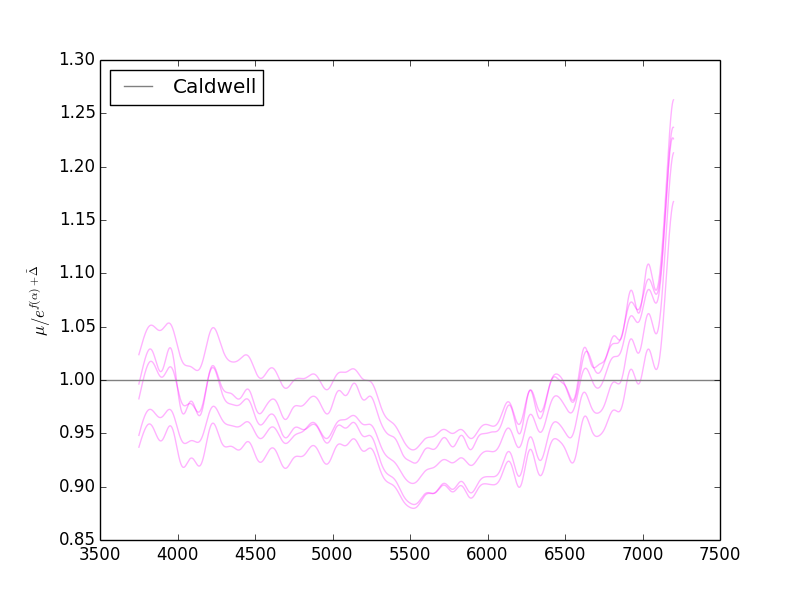
\includegraphics[width=\textwidth]{figures/cfig_b192-g242_225.png}
\caption{Left: Samples of the effective multiplicative calibration
vector for the spectrophotometrically calibrated spectrum of
\excluster~ ({\it cyan}) compared to that obtained from ancillary
photometric data ({\it magenta}).  
%Right: The same, but for the uncalibrated data.
 \label{fig:inferred_calib}}
\end{figure*}


\begin{figure}[h!]
%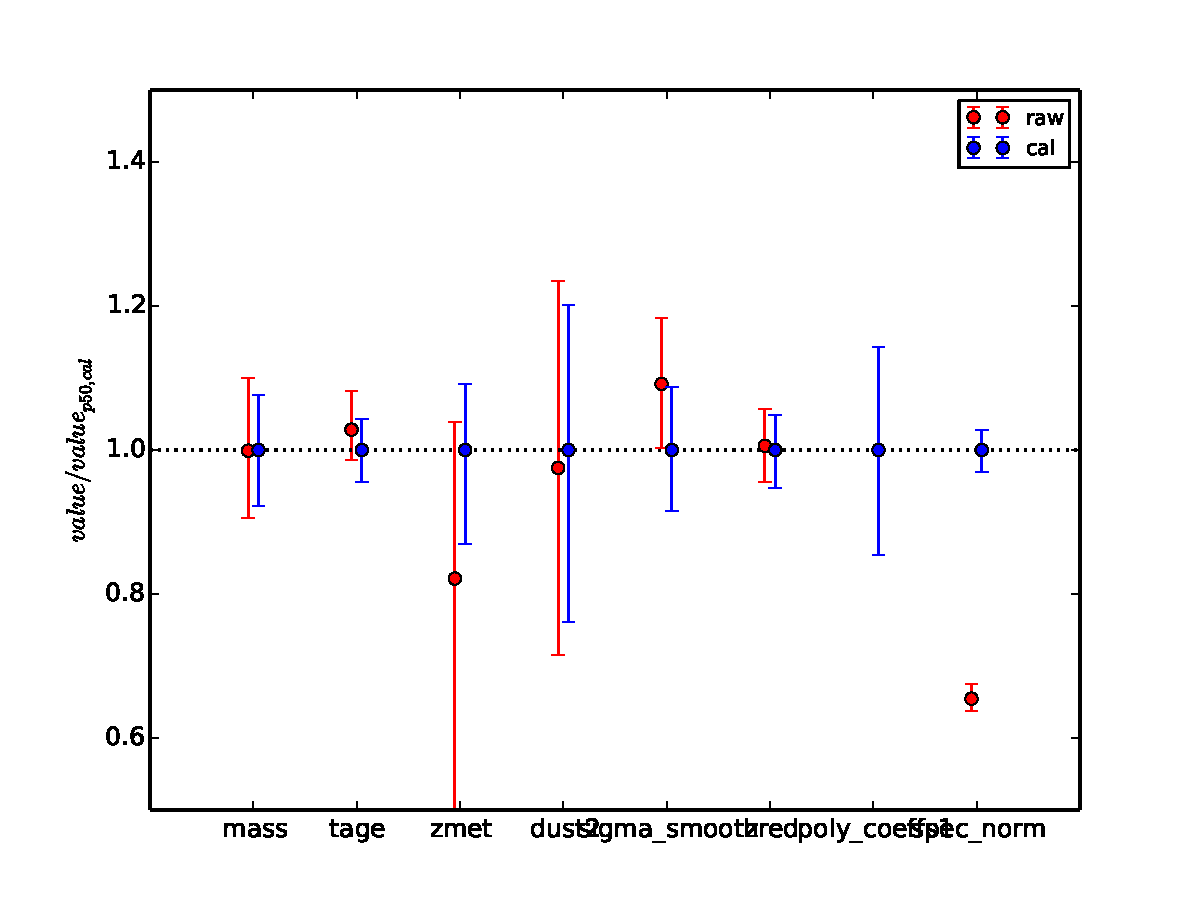
\includegraphics[width =0.5\textwidth]{figures/B192_020_cratio.pdf}
\caption{Money plot.  Show the difference between the parameters
  inferred from the calibrated and uncalibrated spectra, for each
  cluster. Tjis is a placeholder, since it only shows B192 for fixed
  GP parameters. \label{fig:boom}}
\end{figure}

\subsection{Dependence on Photometric Data}
In this section we examine how the constraints on physical (and
calibration) parameters vary as a function of the number and type of
photometric points available. {\color{red} BDJ DO THIS TEST.}

\section{Discussion}

We have demonstrated, using a sample of stellar clusters in M31, that
we can combine photometric and spectroscopic data in a principled way
to infer physical properties.  We do not resort to an arbitrary
down-weighting or up-weighting of certain data. Instead, we explicitly
model our uncertain knowledge of the spectral calibration and infer
this calibration jointly with the physical properties. For a number of
applications this combination of spectroscopy and photometry reduces
the need for spectrophotometric calibration entirely, such that the less
expensive photometric calibration is sufficient.  Additional calibration
information, if it exists, can be incorporated into informative priors
on the calibration parameters of the model, inform the construction
of the calibration model, or approximately remove gross features
that are difficult to model parameterically or as a sum of Gaussians.

{\color{blue} BDJ words about the gains that might be made by
including photometry over a large range in wavelngth with spectroscopy
over relatively small ranges.}

Our strategy is easily extensible to more complicated models, which
include for example night sky-line emission in the spectroscopy (or
residuals from an intial sky-line subtraction), and uncertainties in
wavelength calibration. Furthermore, more complex physical models may
be considered for the mean object model, for example including SFH
parameters so as to model galaxies.  {\color{blue} DISCUSS MORE
COMPLICATED COVARIANCE KERNELS, MULTIPLE KERNELS, etc.  MODEL
CHECKING. As I understand it, additional `bad lines' in the mean model
could be accounted for using narrow quadratics in the covariance
matrix, though their interpretation would be hellish. The best way is
probably to explictly model them in the mean model}

In a heirarchical modelling context it should be possible to use the
inferred calibration parameters, along with additional information
about the observations (e.g. airmass, instrument temperature), to in
turn infer the parameters of a generative model for the calibration
\citep[e.g.][]{spectrophot}. This generative model can then be used in
the (probabilistic) calibration of objects where the spectra are
difficult to model explicitly.

Limitations.  The strategy we have advocated has several limitations.
First, it requires a generative model for the spectrum of the object
of interest, and is thus ill-suited to discovery projects.  Second,
care must be taken to avoid absorbing interesting model deficiencies
into the calibration model. For example, in the model we have
described, it is possible that broad shallow features (for example due
to molecular bands or absorption line complexes) will be absorbed into
the Gaussian process. Third, we have made the assumption that the
spectroscopy and the photometry are sampling the same populations.  In
practice, differences between spectroscopic and photometric apertures
often mean that the photometry and the spectroscopy are sampling
slightly different physical regions.  The correct response to this
situation is to explicitly model the differences, incorporating prior
information about the spatial variation of physical properties.
Fourth, the method will break down at very low S/N due to the
logarithmic formulation of the residual in
equation~(\ref{eq:spectroscopicLF}).  Finally, this method is
computationally intensive and expensive, since we are constantly
inverting largish matrices.

{\color{blue} BDJ - This paragraph is probably too calibration
focused. We want to focus more on spec + phot combinations.  At least,
this paragraph should not be in the discussion section.}
Fundamentally, calibration involves observing a `known' or `truth'
with an instrument, and using that observation to infer the effects of
the instrument.  However, we do not have knowledge of a single truth
for any object, only relative probabilities for what might be true.
In this sense, one should never use a single point estimate of the
calibration, the full distribution of the possible calibrations should
be inferred from our probabilistic knowledge of the calibration object
and forward propogated \citep[e.g.][]{lee11}. Once this is done, the
only distinction between 'calibration' objects and targets of interest
is the complexity of the model for the object and the level of
uncertainty in the calibration object spectrum.  If one is interested
in inferring parameters of interest of spectral models of
astrophysical objects, then there is often no reason not to use those
objects themselves as calibration objects.

BDJ misc issues, collected here in case we want to address them and to
keep me from cluttering up the main text: Model resolution and
instrument resolution.  How to interpret GP residuals, as a fn of S/N?
Photometric upper limits? Infer the wavelength solution as well -
stellar population (and telluric lines) as your arc. Combinations of
broadening in velocity space (physical) and in wavelength space
(instrumental)

HOGG COMPUTE TOTAL ANNUAL COST OF SPECTROPHOTOMETRY (to astronomical community).

All the code used in this project is available under an open-source license
  from \url{http://github.com/bd-j/bsfh/}.
This version of the paper was generated
  from a git repository available at \url{http://github.com/bd-j/speccal/}
  with git hash \texttt{\githash\,(\gitdate)}.

\acknowledgements
Thanks to X. for bringing us beer.
DRW is supported by NASA through Hubble Fellowship grant
  HST-HF-51331.01 awarded by the Space Telescope Science Institute.
BDJ and DRW acknowledge the hospitality of Hans-Walter Rix and the MPIA. 
CC is supported by Packard and Sloan Foundation Fellowships. 
This research made extensive use of NASA's Astrophysics Data System Bibliographic Services. 
In large part, analysis and plots presented in this paper utilized
  iPython and packages from NumPy, SciPy, and Matplotlib
  \citep[][]{hunter2007, oliphant2007, perez2007} as well
  as python-FSPS  (\url{http:://github.com/dfm/python-fsps}) .

\newcommand{\arxiv}[1]{\href{http://arxiv.org/abs/#1}{arXiv:#1}}
\begin{thebibliography}{}\raggedright

\bibitem[Beifiori \etal(2011)]{beifiori11} 
Beifiori, A., Maraston, C., Thomas, D., \& Johansson, J.\ 2011, \aap, 531, A109 

\bibitem[Bertelli et al.(1994)]{bertelli94} Bertelli, G., Bressan, A., Chiosi, C., Fagotto, F., \& Nasi, E.\ 1994, \aaps, 106, 275 

\bibitem[Cardelli \etal(1989)]{CCM89} 
Cardelli, J.~A., Clayton, G.~C., \& Mathis, J.~S.\ 1989, \apj, 345, 245 

\bibitem[Cenarro \etal(2007)]{miles_II} 
Cenarro, A.~J., Peletier, R.~F., S{\'a}nchez-Bl{\'a}zquez, P., et al.\ 2007, \mnras, 374, 
664 

\bibitem[Conroy \etal(2009)]{fsps} 
Conroy, C., Gunn, J.~E., \& White, M.\ 2009, \apj, 699, 486 

\bibitem[Conroy \& Gunn(2010)]{fsps_cal} 
Conroy, C., \& Gunn, J.~E.\ 2010, \apj, 712, 833 

\bibitem[Fabricant \etal(2013)]{fabricant13} 
Fabricant, D., Chilingarian, I., Hwang, H.~S., et al.\ 2013, \pasp, 125, 1362 

\bibitem[Falc{\'o}n-Barroso \etal(2011)]{miles_III} 
Falc{\'o}n-Barroso, J., S{\'a}nchez-Bl{\'a}zquez, P., Vazdekis, A., et al.\ 2011, \aap, 532, A95 

\bibitem[Foreman-Mackey \etal(2012)]{emcee}
Foreman-Mackey, D., Hogg, D.~W., Lang, D., \& Goodman, J.\ 2013, \pasp, 125,
306 (\arxiv{1202.3665})

\bibitem[Girardi et al.(2000)]{girardi00} 
Girardi, L., Bressan, A., Bertelli, G., \& Chiosi, C.\ 2000, \aaps, 141, 371 

\bibitem[Goodman~\&\ Weare(2010)]{goodman}
Goodman,~J. \& Weare,\ J., 2010, Comm.\ App.\ Math.\ Comp.\ Sci., 5, 65

\bibitem[Lee et al.(2011)]{xray_calunc} Lee, H., Kashyap, V.~L., 
van Dyk, D.~A., et al.\ 2011, \apj, 731, 126 

\bibitem[Marigo \& Girardi(2007)]{marigo07} 
Marigo, P., \& Girardi, L.\ 2007, \aap, 469, 239 

\bibitem[S{\'a}nchez-Bl{\'a}zquez \etal(2006)]{miles_I} 
S{\'a}nchez-Bl{\'a}zquez, P., Peletier, R.~F., Jim{\'e}nez-Vicente,
J., et  al.\ 2006, \mnras, 371, 703 


\end{thebibliography}

\end{document}
